\documentclass{beamer}
\usepackage{amsfonts,amsmath,oldgerm}  % rimosso enumitem
\usetheme{sintef}
\usepackage{tikz}
\usetikzlibrary{positioning}
\usepackage{booktabs}
\usepackage{appendixnumberbeamer}
\usepackage{colortbl}
\definecolor{darkblue}{RGB}{0,51,102}

\newcommand{\testcolor}[1]{\colorbox{#1}{\textcolor{#1}{test}}~\texttt{#1}}
\definecolor{azzurro}{HTML}{AED6F1}
\definecolor{azzurroborder}{HTML}{2E86C1}
\usefonttheme[onlymath]{serif}

\titlebackground*{assets/background}

\newcommand{\hrefcol}[2]{\textcolor{cyan}{\href{#1}{#2}}}

\title{DNA Methylation Dynamics Along\\[-5pt]the Normal–Adjacent Axis in\\Breast Cancer}
\subtitle{A Quantitative Statistical and Machine Learning Approach}
\course{Laurea Magistrale in Ingegneria Matematica}
\author{\href{mailto:elisabetta.roviera@studenti.polito.it}{Elisabetta ROVIERA}}
\IDnumber{328422}
\date{%
  \vspace{1.5pt}
  Relatori: Prof. Alfredo BENSO \\
  \phantom{Relatori: }Dott. Sandro GAMBINO \\
  16 Marzo 2026%
}

\begin{document}

\maketitle

\section{Dal Problema Biologico ai Dati}

\begin{frame}{Il Tumore al Seno: una Sfida Globale}

\begin{columns}[T]

  % COLONNA SINISTRA — incidenza
  \begin{column}{0.48\textwidth}
    \centering
    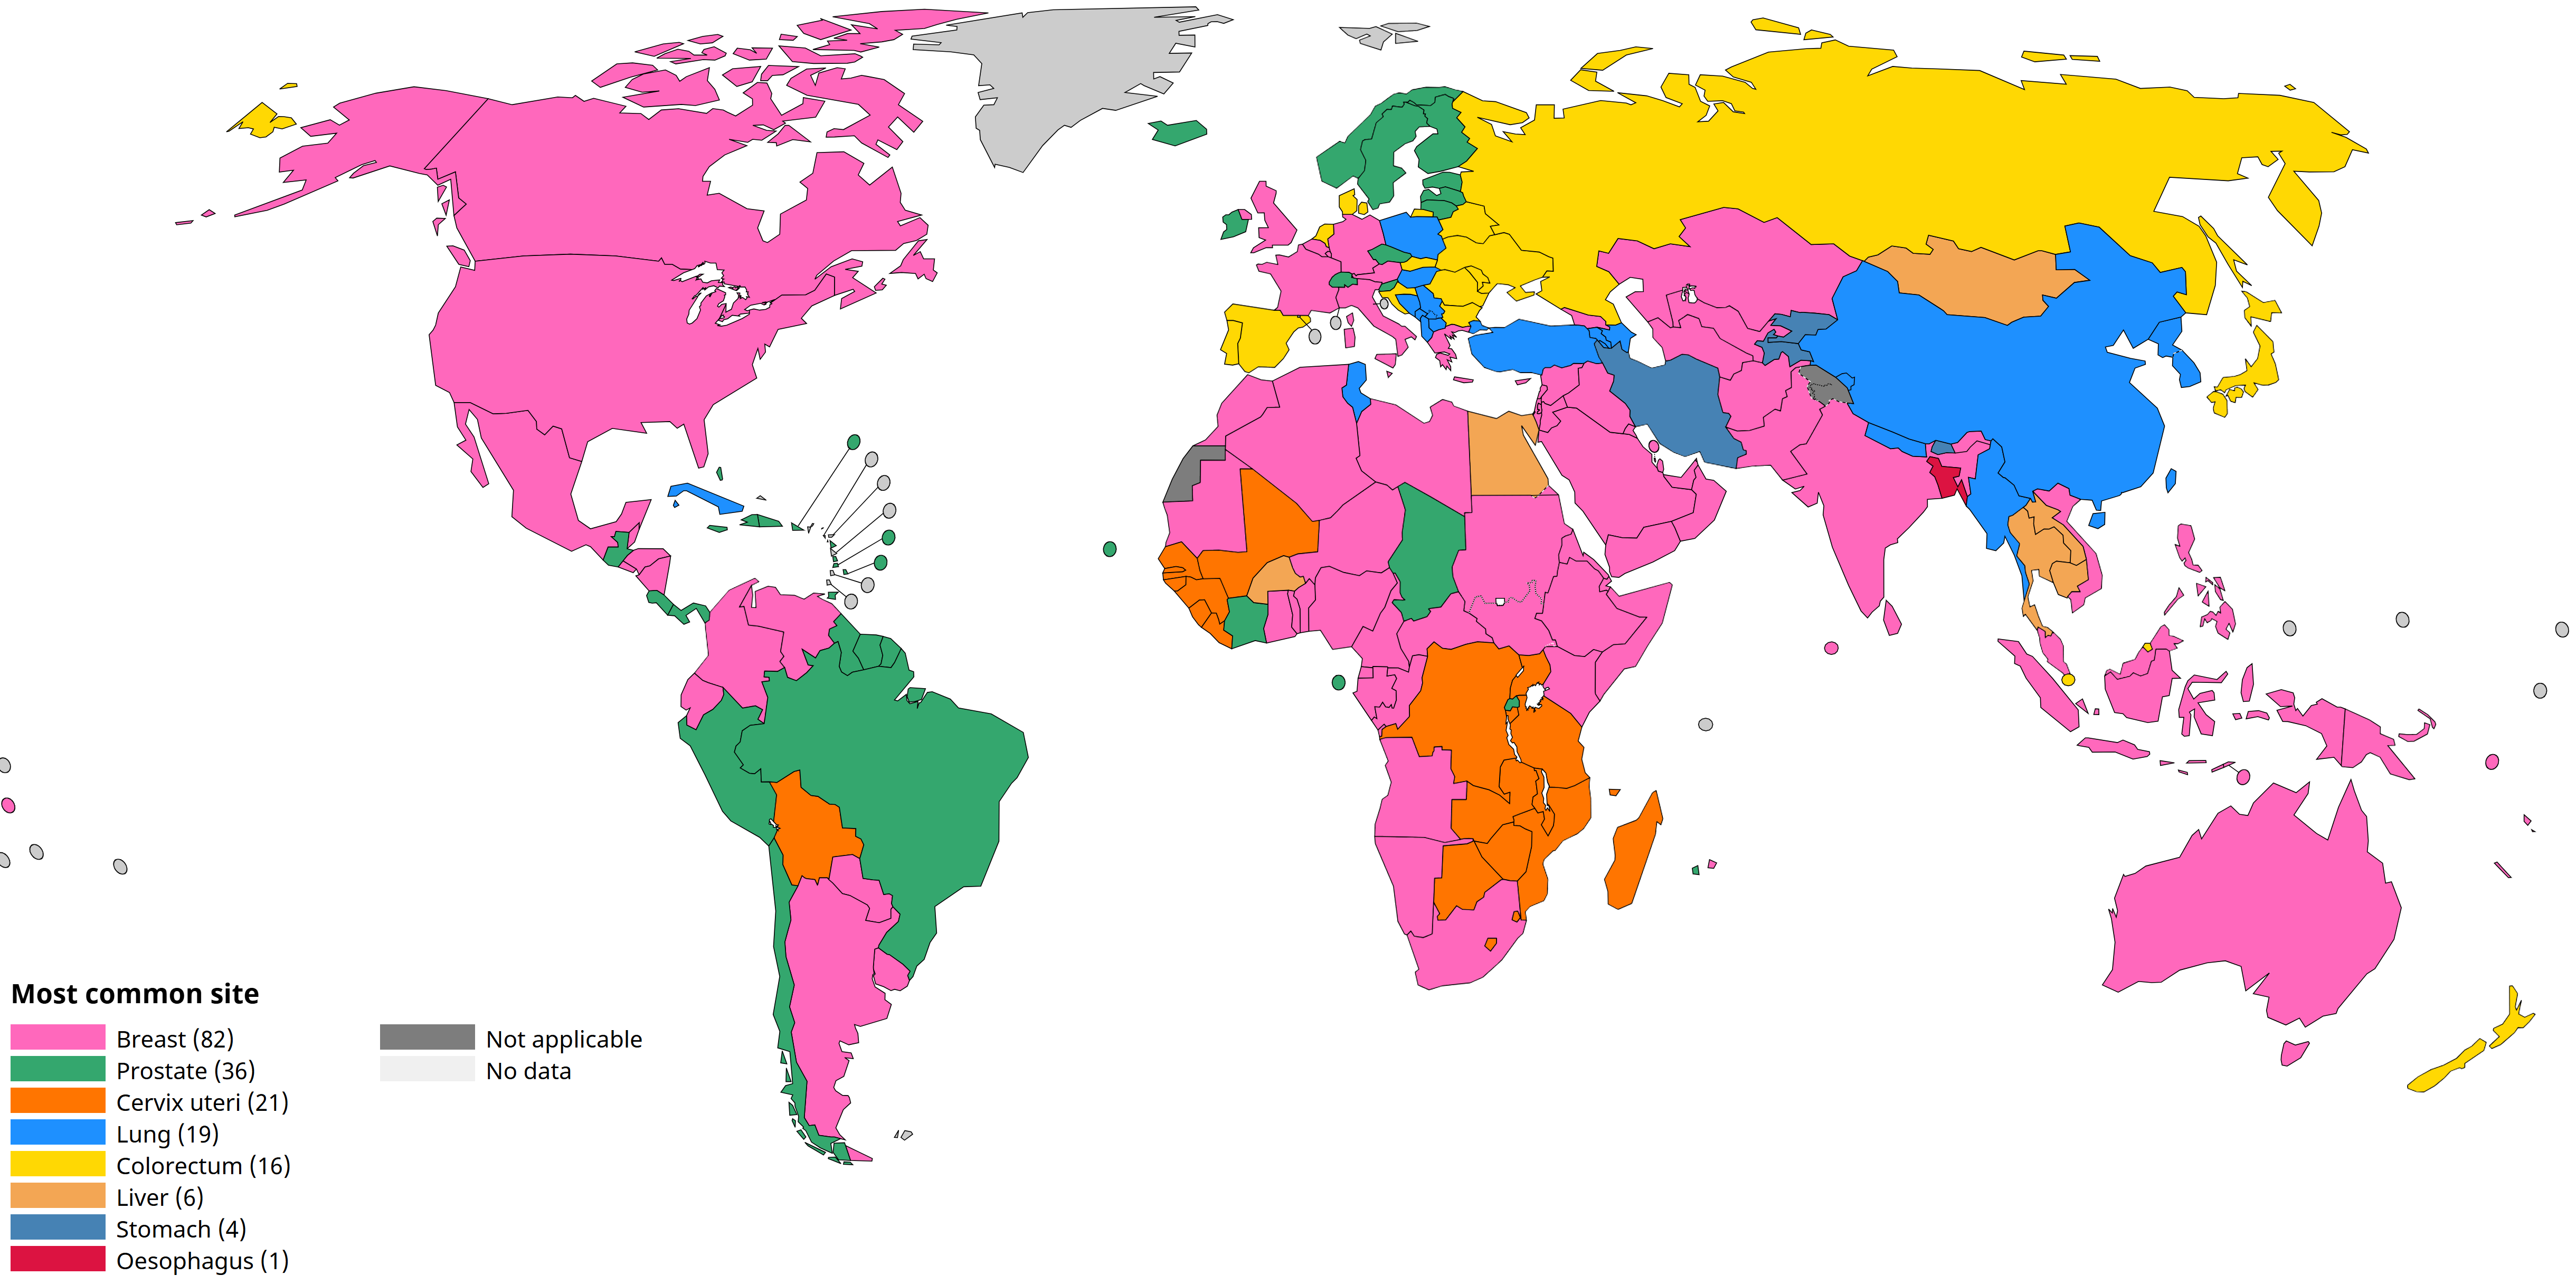
\includegraphics[height=3.2cm]{images/impatto.png}
    
    {\scriptsize \textit{Tumore più comune per paese — GLOBOCAN 2022 \\ In rosa è riportato il tumore al seno}}
    
    \vspace{4pt}
    
    \begin{itemize}
      \item[\textbf{--}] \textbf{2.3 milioni} di nuovi casi
      \item[\textbf{--}] Più diagnosticato in \textbf{82 su 185} paesi
    \end{itemize}

  \end{column}

  % COLONNA DESTRA — field cancerization
  \begin{column}{0.48\textwidth}
    \centering
    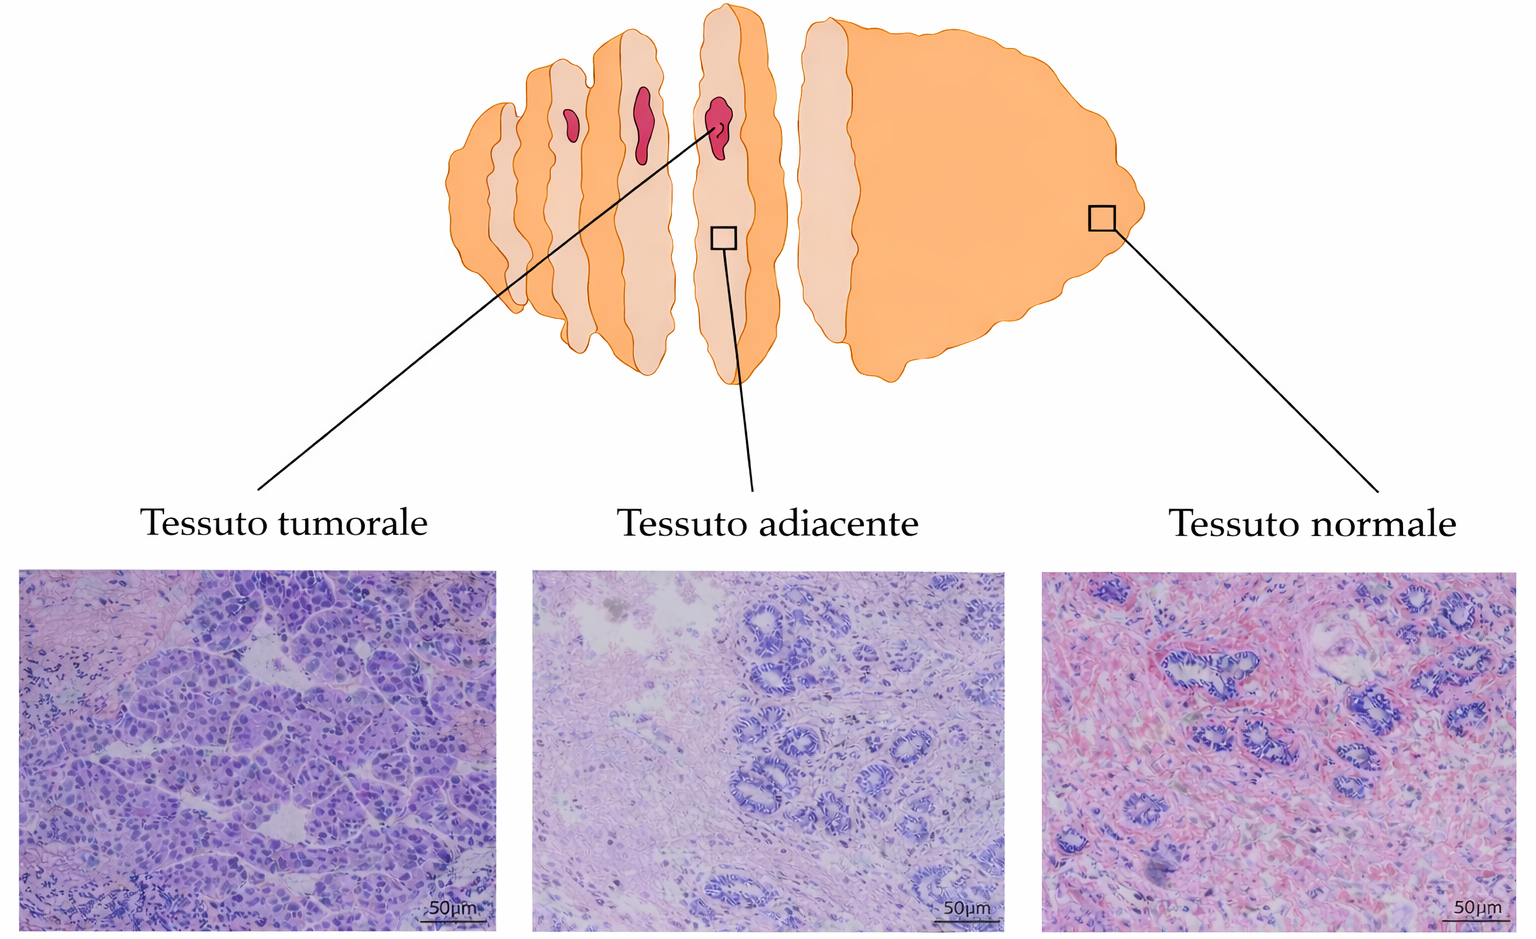
\includegraphics[height=3.1cm]{images/field_cancerisation.png}
    
    {\scriptsize \textit{Tessuto tumorale, adiacente e normale a confronto — Gadaleta et al., J Pathol, 2022}}\\
    
    \vspace{4pt}
    
    \begin{itemize}
      \item[\textbf{--}]  \textbf{Distinguere} Normale da Adiacente per studiare le \textbf{alterazioni epigenetiche precoci}
    \end{itemize}
  \end{column}

\end{columns}

\end{frame}

\begin{frame}{Metilazione del DNA: Segnale Biologico e Statistico}

\begin{columns}[T]
  \begin{column}{0.48\textwidth}
    \centering
    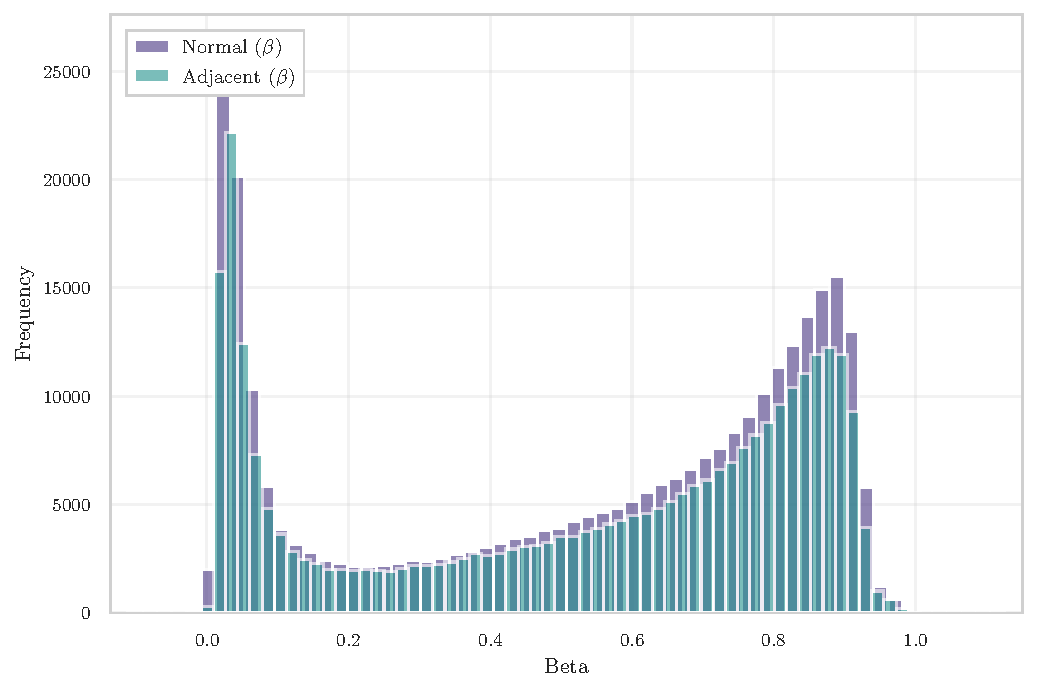
\includegraphics[height=3.9cm]{images/beta_normal_vs_adjacent.pdf}\\[2pt]
    {\scriptsize $\beta$-value $\in [0,1]$\\[2pt]}
  \end{column}
  \begin{column}{0.48\textwidth}
    \centering
    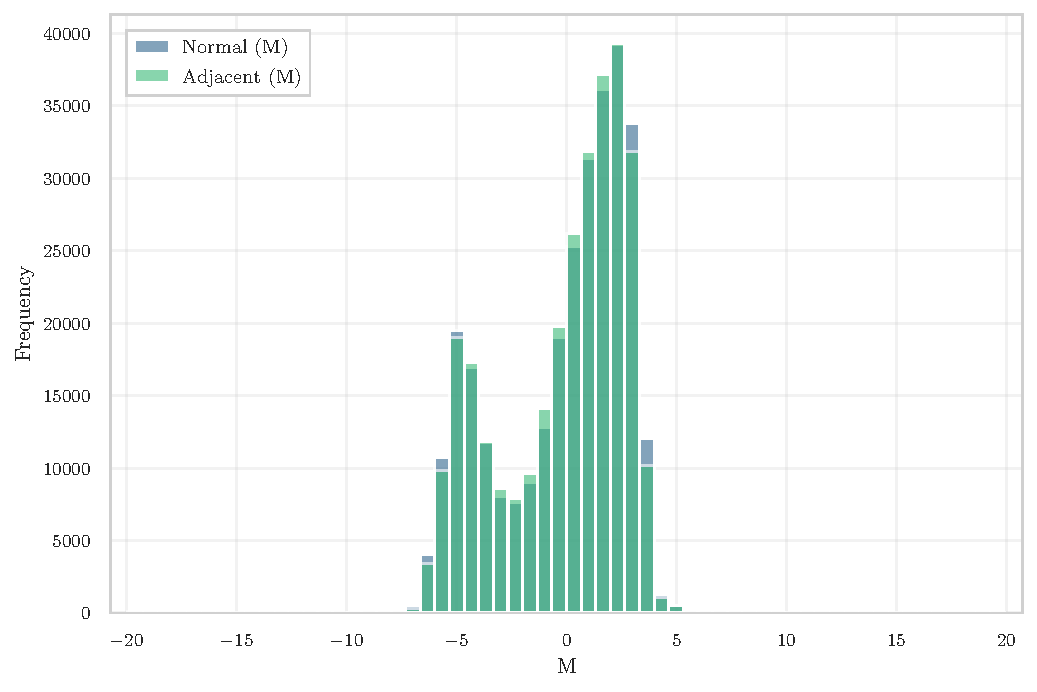
\includegraphics[height=3.9cm]{images/m_normal_vs_adjacent.pdf}\\[2pt]
    {\scriptsize $M = \log_2\!\left(\frac{\beta}{1-\beta}\right) \in (-\infty, +\infty)$\\[2pt]}
  \end{column}
\end{columns}

\vspace{12pt}

{\small
\begin{columns}[T]
  \begin{column}{0.48\textwidth}
    \textbf{Metilazione del DNA}\\[3pt]
    \quad -- \textbf{Ipermetilazione} $\rightarrow$ gene silenziato\\
    \quad -- \textbf{Ipometilazione} $\rightarrow$ gene attivo
  \end{column}
  \begin{column}{0.48\textwidth}
    \textbf{Illumina EPIC} $\sim$\textbf{866k} siti CpG\\[3pt]
    \quad -- \textbf{295} Normali\\
    \quad -- \textbf{200} Adiacenti
  \end{column}
\end{columns}
}

\end{frame}

\section{Dal Dato Grezzo alla Feature Selection}

\begin{frame}{Preprocessing: dal Rumore al Segnale}

\begin{columns}[T]
  \begin{column}{0.32\textwidth}
    \centering
    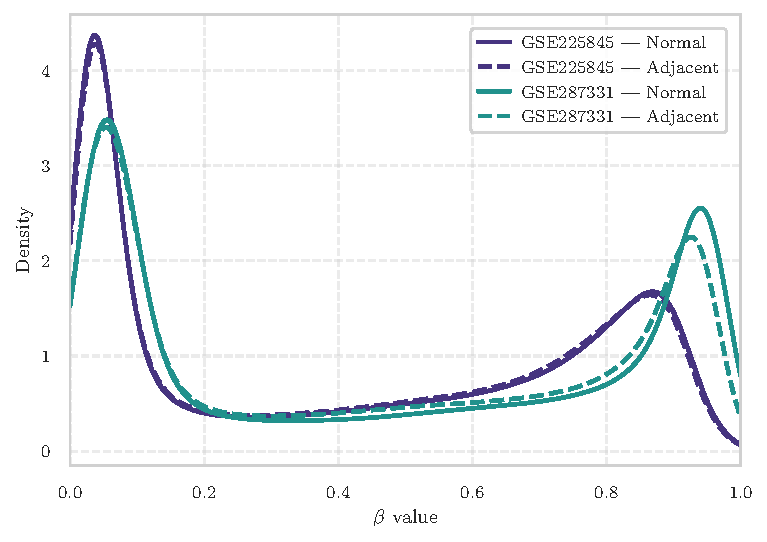
\includegraphics[width=\textwidth]{images/plot_raw_beta.pdf}\\[2pt]
    {\scriptsize $\beta$-value grezzo \\ Segnale biologico
    e tecnico sovrapposti}
  \end{column}
  \begin{column}{0.32\textwidth}
    \centering
    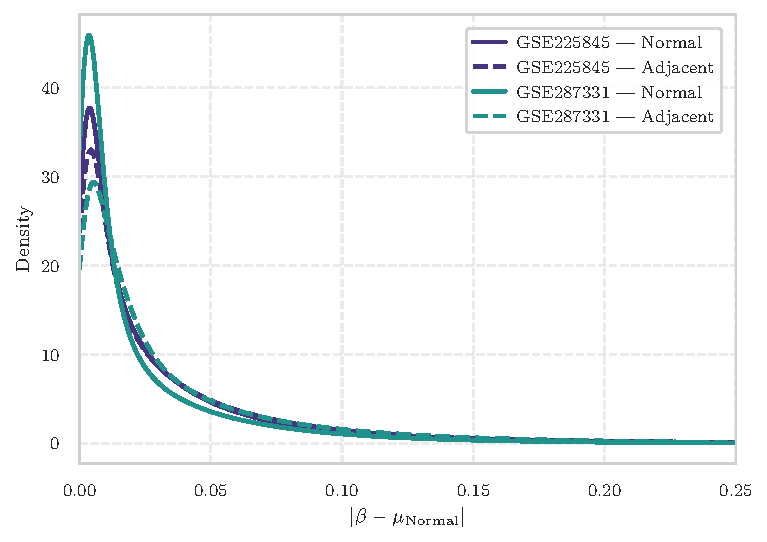
\includegraphics[width=\textwidth]{images/plot_abs_deviation.pdf}\\[2pt]
    {\scriptsize Post-$|\beta_{ij} - \bar{\beta}^{\text{Normal}}_j|$\\Deviazione
    dal tessuto sano amplificata}
  \end{column}
  \begin{column}{0.32\textwidth}
    \centering
    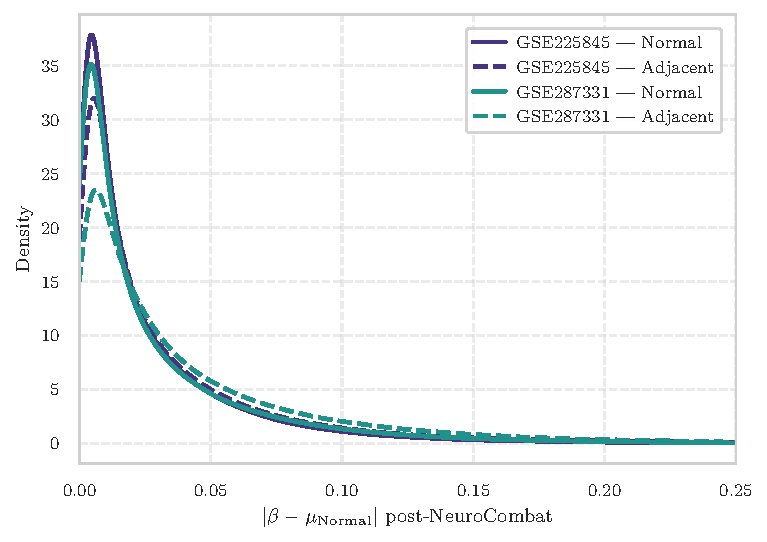
\includegraphics[width=\textwidth]{images/plot_postcombat.pdf}\\[2pt]
    {\scriptsize Post-NeuroCombat\\
    Batch rimosso, segnale preservato}
  \end{column}
\end{columns}

\end{frame}

\begin{frame}{Riduzione dello Spazio delle Feature}

\begin{center}
\begin{tikzpicture}[
  node distance=0.30cm,
  base/.style={
    rectangle, rounded corners=3pt,
    minimum width=8.8cm, minimum height=0.58cm,
    text centered, font=\small, inner sep=4pt,
  },
  n0style/.style={base, draw=maincolor, fill=maincolor!20},
  n1style/.style={base, draw=maincolor!40, fill=maincolor!6},
  filterstyle/.style={base, draw=maincolor!60, fill=maincolor!10},
  hlstyle/.style={base, font=\small\bfseries,
    draw=sinteflightgreen!80!black, fill=sinteflightgreen!25},
  arrow/.style={->, thick, color=gray!40, shorten >=1pt, shorten <=1pt}
]

\node[n0style]     (n0) {Feature Iniziali \hspace{0.8cm} $\rightarrow$ \hspace{0.4cm} \textbf{866,552} CpG};
\node[n1style,     below=of n0] (n1) {Pre-processing \hspace{0.8cm} $\rightarrow$ \hspace{0.4cm} \textbf{485,453} CpG};
\node[filterstyle, below=of n1] (n2) {Filtro variabilità \hspace{0.8cm} $\rightarrow$ \hspace{0.4cm} \textbf{284,310} CpG};
\node[filterstyle, below=of n2] (n3) {Filtro varianza \hspace{0.8cm} $\rightarrow$ \hspace{0.4cm} \textbf{270,094} CpG};
\node[hlstyle,     below=of n3] (n4) {Stability ranking \hspace{0.8cm} $\rightarrow$ \hspace{0.4cm} \textbf{15,659} CpG};
\node[hlstyle,     below=of n4] (n5) {Correlation pruning \hspace{0.8cm} $\rightarrow$ \hspace{0.4cm} \textbf{15,523} CpG};
\node[filterstyle, below=of n5] (n6) {Diversificazione genomica vincolata \hspace{0.8cm} $\rightarrow$ \hspace{0.4cm} \textbf{5,000} CpG};

\draw[arrow] (n0.south) -- (n1.north);
\draw[arrow] (n1.south) -- (n2.north);
\draw[arrow] (n2.south) -- (n3.north);
\draw[arrow] (n3.south) -- (n4.north);
\draw[arrow] (n4.south) -- (n5.north);
\draw[arrow] (n5.south) -- (n6.north);

\end{tikzpicture}
\end{center}

\vspace{0.4em}
\hfill{\scriptsize $\rightarrow$ Step completi in appendice.}


\end{frame}

\begin{frame}{Stability Ranking}

\begin{center}
\begin{tikzpicture}[
  top/.style={rectangle, rounded corners=3pt,
    minimum width=8.0cm, minimum height=0.52cm,
    align=center, font=\small,
    draw=maincolor!40, fill=maincolor!6},
  stat/.style={rectangle, rounded corners=3pt,
    minimum width=3.8cm,
    align=center, font=\scriptsize, inner sep=7pt,
    draw=sinteflightgreen!80!black, fill=sinteflightgreen!25},
  bio/.style={rectangle, rounded corners=3pt,
    minimum width=3.8cm,
    align=center, font=\scriptsize, inner sep=7pt,
    draw=maincolor!60, fill=maincolor!10},
  cutoff/.style={rectangle, rounded corners=3pt,
    minimum width=8.0cm, minimum height=0.52cm,
    align=center, font=\scriptsize,
    draw=maincolor!40, fill=maincolor!6},
  sel/.style={rectangle, rounded corners=3pt,
    minimum width=8.0cm, minimum height=0.52cm,
    align=center, font=\small\bfseries,
    draw=maincolor, fill=maincolor!20},
  arrow/.style={->, thick, color=gray!50,
    shorten >=1pt, shorten <=1pt}
]

\node[top]    (input)  at (0, 0.0)
  {\textbf{270,094} CpG candidati};

\node[top]    (score)  at (0,-0.85)
  {$\text{score} = \tfrac{1}{2}\;\text{score\_stat} + \tfrac{1}{2}\;\text{score\_bio}$};

\node[stat] (stat0) at (-2.8,-3.1)
  {$\text{score\_stat}_i = \tfrac{1}{2}\,\overline{\text{rank}}_{p,i}
    + \tfrac{1}{2}\,\overline{\text{rank}}_{|\Delta M|,i}$\\[6pt]
   $\overline{\text{rank}}_{p,i} = 
     p\text{-value}_{i}$\\[5pt]
   $\overline{\text{rank}}_{|\Delta M|,i} = 
     |\bar{M}^i_{\text{ad}} - \bar{M}^i_{\text{no}}|$\\[3pt]
};

\node[bio] (bio0) at (2.8,-3.1)
  {$\text{score\_bio}_i = \tfrac{1}{2}(1\!-\!\text{IP}_i)
    + \tfrac{1}{2}(1\!-\!\text{bio\_w}_i)$\\[6pt]
   $\text{IP}_i = \dfrac{\bar{M}^i_{\text{ad}} - \bar{M}^i_{\text{no}}}%
                        {\bar{M}^i_{\text{tum}} - \bar{M}^i_{\text{no}}}$\\[5pt]
   bio\_w$_i$: posizione genomica};
\node[cutoff] (cut)    at (0,-5.2)
  {stabilità del segno \textbf{e}
   soglia data-driven su $|\Delta M|$};

\node[sel]    (output) at (0,-6.0)
  {\textbf{15,659} CpG — ordinati per score};

\draw[arrow] (input)       -- (score);
\draw[arrow] (score.south) -- ++(0,-0.25) -| (stat0.north);
\draw[arrow] (score.south) -- ++(0,-0.25) -| (bio0.north);
\draw[arrow] (stat0.south) -- ++(0,-0.25) -| (cut.north);
\draw[arrow] (bio0.south)  -- ++(0,-0.25) -| (cut.north);
\draw[arrow] (cut)         -- (output);

\end{tikzpicture}
\end{center}

\end{frame}


\begin{frame}{Correlation Pruning tramite Grafi}

\begin{columns}[T]

  % COLONNA SINISTRA — schema grafo
  \begin{column}{0.44\textwidth}
    \centering
    \vspace{6pt}
    \begin{tikzpicture}[
      cpg/.style={circle, draw=maincolor, fill=maincolor!15,
                  minimum size=0.45cm, inner sep=1pt},
      rep/.style={circle, draw=maincolor, fill=maincolor!50,
                  minimum size=0.45cm, inner sep=1pt},
      edge/.style={thick, color=maincolor!70},
      arr/.style={->, thick, color=gray!50}
    ]
      \node[rep]  (a1) at (0,0)     {};
      \node[cpg]  (a2) at (0.9,0.4) {};
      \node[cpg]  (a3) at (0.9,-0.4){};
      \node[cpg]  (a4) at (1.8,0)   {};
      \draw[edge] (a1)--(a2);
      \draw[edge] (a1)--(a3);
      \draw[edge] (a2)--(a4);
      \draw[edge] (a3)--(a4);

      \node[rep]  (b1) at (3.0, 0.4) {};
      \node[cpg]  (b2) at (3.9, 0.4) {};
      \draw[edge] (b1)--(b2);

      \node[rep]  (c1) at (3.45,-0.4) {};

      \node[font=\scriptsize, text=maincolor] at (0.9,-0.9)
        {componente 1};
      \node[font=\scriptsize, text=maincolor, align=center] at (3.45, 0.9)
        {componente 2};
      \node[font=\scriptsize, text=maincolor, align=center] at (3.45,-0.9)
        {componente 3};

      \draw[arr] (1.8,-1.3) -- (1.8,-1.8);

      \node[rep] (r1) at (0.6,-2.2) {};
      \node[rep] (r2) at (1.8,-2.2) {};
      \node[rep] (r3) at (3.0,-2.2) {};

      \node[font=\scriptsize, align=center] at (1.8,-2.8)
        {1 rappresentante per componente\\
         {\tiny (score minimo nel cluster)}};

    \end{tikzpicture}

    \vspace{2pt}
    {\scriptsize Arco se $|r| \geq 0.85$}
  \end{column}

  % COLONNA DESTRA — biforcazione Pool A / Pool B
  \begin{column}{0.52\textwidth}
    \centering
    \vspace{4pt}
    \begin{tikzpicture}[
      box/.style={rectangle, rounded corners=2pt, minimum width=2.6cm,
                  minimum height=0.55cm, align=center, font=\small,
                  draw=maincolor!40, fill=maincolor!6},
      boxa/.style={rectangle, rounded corners=2pt, minimum width=2.6cm,
                   minimum height=0.55cm, align=center, font=\small,
                   draw=sinteflightgreen!80!black, fill=sinteflightgreen!25},
      boxb/.style={rectangle, rounded corners=2pt, minimum width=2.6cm,
                   minimum height=0.55cm, align=center, font=\small,
                   draw=maincolor!60, fill=maincolor!10},
      final/.style={rectangle, rounded corners=2pt, minimum width=3.4cm,
                    minimum height=0.55cm, align=center, font=\small\bfseries,
                    draw=maincolor, fill=maincolor!20},
      arr/.style={->, thick, color=gray!50}
    ]

      \node[box] (top) at (1.5, 0) {\textbf{15,659} CpG candidati};

      \node[boxa] (pa) at (0.0,-1.0)
        {\textbf{Pool A} --- island \\ {\scriptsize 1,937 CpG}};
      \node[boxb] (pb) at (3.0,-1.0)
        {\textbf{Pool B} --- resto \\ {\scriptsize 13,722 CpG}};

      \draw[arr] (top) -- (pa);
      \draw[arr] (top) -- (pb);

      \node[boxa] (ra) at (0.0,-2.1)
        {pruning $|r|\geq0.85$ \\ {\scriptsize 1,888 CpG}};
      \node[boxb] (rb) at (3.0,-2.1)
        {pruning $|r|\geq0.85$ \\ {\scriptsize 12,952 CpG}};

      \draw[arr] (pa) -- (ra);
      \draw[arr] (pb) -- (rb);

      \node[final] (fin) at (1.5,-3.2) {\textbf{15,523} CpG};

      \draw[arr] (ra) -- (fin);
      \draw[arr] (rb) -- (fin);

    \end{tikzpicture}

    \vspace{2pt}
    {\scriptsize Pool A: CpG ancorati a \textit{CpG islands} (biologicamente privilegiati)\\
    Pool B: restanti CpG candidati}
  \end{column}

\end{columns}

\end{frame}


\section{Dal MILP alla Soluzione}


\begin{frame}{Selezione delle CpG Finali: MILP Knapsack}
{\scriptsize
\begin{alignat*}{3}
\max_{x} \quad
& \sum_{j \in \mathcal{J}} v_j\, x_j \;+\; \mu \cdot \hat{\Phi}(x, y) & & \\[6pt]
\text{s.t.} \quad
& \sum_{j \in \mathcal{J}} x_j = 50
  &\qquad& \textbf{(Cardinalità)} \\[4pt]
& \sum_{j \in \mathcal{J}_c} x_j \leq 10 \quad \forall\, c
  &\qquad& \textbf{(Bilanciamento cromosomico)} \\[4pt]
& \sum_{j:\,g(j)=g} x_j \leq 2 \quad \forall\, g
  &\qquad& \textbf{(Max CpG per gene)} \\[4pt]
& x_j \leq y_{g(j)} \leq \textstyle\sum_{j':\,g(j')=g} x_{j'} \quad \forall\, j : g(j) \neq \emptyset
  &\qquad& \textbf{(Gene linking)} \\[4pt]
& x_i + x_j \leq 1 \quad \forall\,(i,j):|r_{ij}|\geq 0.85
  &\qquad& \textbf{(Non-ridondanza)} \\[4pt]
& x_j,\, y_g \in \{0,1\}
\end{alignat*}
}

\hfill{\scriptsize $\rightarrow$ Formulazione completa in appendice.}

\end{frame}

\begin{frame}{Risultati: il Trade-off Esplicito}

\begin{columns}[c, onlytextwidth]

% ---------------- LEFT ----------------
\column{0.54\textwidth}
\centering
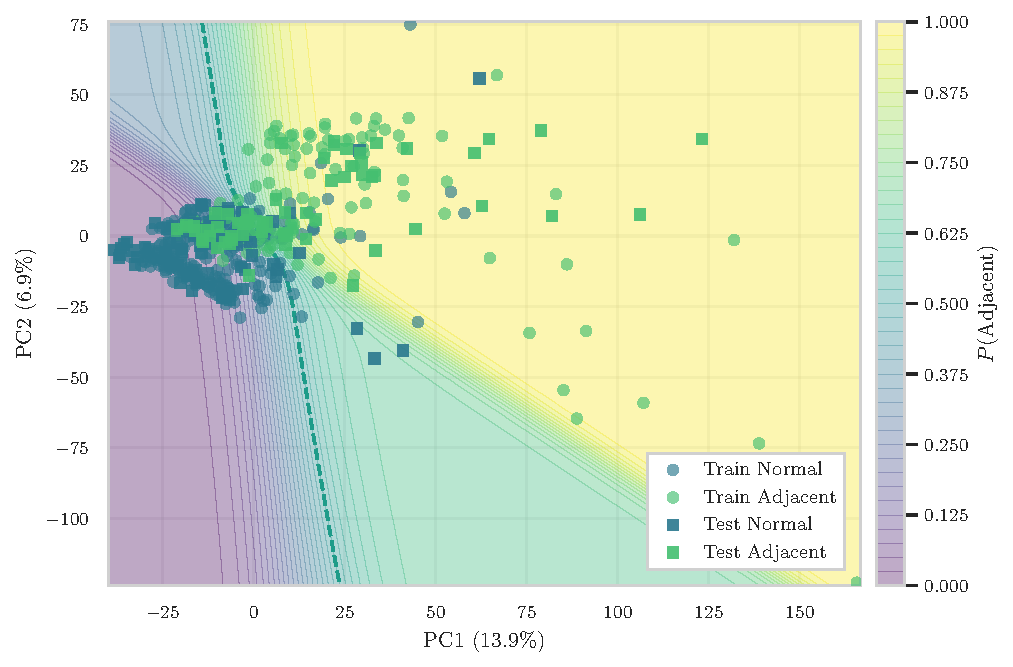
\includegraphics[width=\linewidth]{images/multicohort_boundary_pca_prob_calibrated.pdf}

{\small Decision boundary nello spazio PCA dei 50 CpG selezionati}

% ---------------- RIGHT ----------------
\column{0.46\textwidth}
\centering

\vfill

{\footnotesize
\renewcommand{\arraystretch}{1.3}
\begin{tabular}{lccc}
\toprule
\textbf{Approccio} & \textbf{AUC} & \textbf{BACC} & \textbf{COSMIC} \\
\midrule
Baseline           & 0.952 & 0.90 & 1  \\
Greedy top-50      & 0.982 & 0.92 & 0  \\
\rowcolor{blue!10}
MILP knapsack      & 0.974 & 0.91 & 13 \\
\bottomrule
\end{tabular}
}

\vspace{6pt}

{\scriptsize
\textit{COSMIC}: geni nel Cancer Gene Census\\
con annotazione breast cancer
}

\vfill

\end{columns}

\end{frame}


\begin{frame}{Interpretabilità Biologica}

\begin{columns}[t, onlytextwidth]

\column{0.48\textwidth}

% RB1
\begin{beamercolorbox}[rounded=true, sep=6pt]{block body}
{\large \textcolor{darkblue}{$\blacksquare$}}\;
\textbf{RB1} \hfill {\scriptsize \textit{Tumor suppressor}}\\[3pt]
{\scriptsize
\begin{itemize}
  \setbeamertemplate{itemize item}{\textcolor{darkblue}{$\blacksquare$}}
  \item \textbf{Ruolo:} regolatore principale del ciclo cellulare
  \item \textbf{Rilevanza:} tra i marcatori più consolidati di field cancerization mammaria
\end{itemize}
}
\end{beamercolorbox}

\vspace{0.5em}



% AKT1
\begin{beamercolorbox}[rounded=true, sep=6pt]{block body}
{\large \textcolor{darkblue}{$\blacktriangle$}}\;
\textbf{AKT1} \hfill {\scriptsize \textit{Segnalazione}}\\[3pt]
{\scriptsize
\begin{itemize}
  \setbeamertemplate{itemize item}{\textcolor{darkblue}{$\blacktriangle$}}
  \item \textbf{Ruolo:} kinasi centrale del pathway PI3K/AKT/mTOR
  \item \textbf{Rilevanza:} tra i più alterati nel carcinoma mammario, bersaglio di terapie mirate approvate
\end{itemize}
}
\end{beamercolorbox}

\column{0.48\textwidth}

% NOTCH1
\begin{beamercolorbox}[rounded=true, sep=6pt]{block body}
{\large \textcolor{darkblue}{$\bullet$}}\;
\textbf{NOTCH1} \hfill {\scriptsize \textit{Segnalazione}}\\[3pt]
{\scriptsize
\begin{itemize}
  \setbeamertemplate{itemize item}{\textcolor{darkblue}{$\bullet$}}
  \item \textbf{Ruolo:} mantenimento cellule staminali tumorali
  \item \textbf{Rilevanza:} promuove progressione verso fenotipi invasivi
\end{itemize}
}
\end{beamercolorbox}

\vspace{0.5em}
% TBX3
\begin{beamercolorbox}[rounded=true, sep=6pt]{block body}
{\large \textcolor{darkblue}{$\blacklozenge$}}\;
\textbf{TBX3} \hfill {\scriptsize \textit{Fattore di trascrizione}}\\[3pt]
{\scriptsize
\begin{itemize}
  \setbeamertemplate{itemize item}{\textcolor{darkblue}{$\blacklozenge$}}
  \item \textbf{Ruolo:} regola l'identità cellulare mammaria
  \item \textbf{Rilevanza:} alterazione epigenetica associata a perdita di differenziazione nel carcinoma luminale
\end{itemize}
}
\end{beamercolorbox}


\end{columns}

\vspace{0.4em}
\hfill{\scriptsize $\rightarrow$ Lista completa in appendice.}

\end{frame}

\section{Dalle Conclusioni agli Sviluppi Futuri}

\begin{frame}{Conclusioni}

\vspace{0.5em}
\centering
{\small Le 50 CpG dimostrano che \textbf{performance e interpretabilità
biologica non sono in conflitto}}

\vspace{1em}

\begin{columns}[t, onlytextwidth]

\column{0.23\textwidth}
\centering
{\Large \textcolor{darkblue}{$\blacksquare$}}\\[4pt]
{\footnotesize \textbf{Feature\\Selection}}\\[4pt]
{\scriptsize 866k $\rightarrow$ 5.000 CpG stabili e non ridondanti}

\column{0.23\textwidth}
\centering
{\Large \textcolor{darkblue}{$\blacklozenge$}}\\[4pt]
{\footnotesize \textbf{MILP\\Knapsack}}\\[4pt]
{\scriptsize Biologia come vincolo strutturale}

\column{0.23\textwidth}
\centering
{\Large \textcolor{darkblue}{$\blacktriangle$}}\\[4pt]
{\footnotesize \textbf{Pannello\\50 CpG}}\\[4pt]
{\scriptsize AUC 0.974 \\ 13 geni COSMIC breast}

\column{0.23\textwidth}
\centering
{\Large \textcolor{darkblue}{$\bullet$}}\\[4pt]
{\footnotesize \textbf{Validazione\\Multi-dataset}}\\[4pt]
{\scriptsize Segnale riproducibile su due coorti EPIC indipendenti}

\end{columns}

\end{frame}

\begin{frame}{Limitazioni e Sviluppi Futuri}

\vspace{1em}

\begin{columns}[t, onlytextwidth]

\column{0.48\textwidth}
\centering
{\large \textcolor{darkblue}{$\triangledown$}}\\[4pt]
{\footnotesize \textbf{Limitazioni}}\\[0.8em]

{\scriptsize
\textbf{Validazione esterna}\\
Nessun dataset EPIC indipendente dalla pipeline\\[0.6em]
\textbf{Cross-piattaforma}\\
Mancata trasferibilità a HM450K
}

\column{0.48\textwidth}
\centering
{\large \textcolor{darkblue}{$\blacktriangleright$}}\\[4pt]
{\footnotesize \textbf{Sviluppi Futuri}}\\[0.8em]

{\scriptsize
\textbf{Altri tumori}\\
Framework MILP parametrizzabile per colon, ovaio\\[0.6em]
\textbf{Integrazione multi-omica}\\
RNA-seq per confermare il ruolo funzionale delle CpG
}

\end{columns}

\vspace{1.2em}
\hrule
\vspace{0.8em}

\centering
{\footnotesize \textcolor{darkblue}{$\star$}\quad \textbf{Pubblicazione}}\\[0.4em]
{\scriptsize
Un \textbf{articolo} basato sulla pipeline presentata è sottomesso a\\
\textit{\textbf{IWBBIO 2026} — 13th International Work-Conference on Bioinformatics and Biomedical Engineering}\\
Gran Canaria, Spagna
}

\end{frame}




\backmatter

\appendix

\begin{frame}{Appendice — NeuroCombat}

\begin{columns}[c, onlytextwidth]

% ---- LEFT: formula ----
\column{0.42\textwidth}

{\footnotesize \textbf{Modello di batch correction}}\\[0.6em]

{\small
\[
Y_{ijd} = \alpha_j + X\beta_j + \gamma_{jd} + \delta_{jd}\,\varepsilon_{ijd}
\]
}

\vspace{0.5em}
{\scriptsize
\begin{itemize}\setlength\itemsep{0.4em}
  \item $\alpha_j$ — media globale del CpG $j$
  \item $X\beta_j$ — effetto delle covariate biologiche protette:\\ tissue label + età
  \item $\gamma_{jd}$ — effetto additivo del batch $d$
  \item $\delta_{jd}$ — effetto moltiplicativo del batch $d$
  \item $\gamma_{jd},\,\delta_{jd}$ stimati via \textbf{Empirical Bayes shrinkage}
\end{itemize}

\vspace{0.4em}
Parametri stimati \textbf{solo su train}; applicati al test via \texttt{neuroCombatFromTraining} — zero leakage.
}

% ---- RIGHT: plot pre/post ----
\column{0.55\textwidth}

\centering

{\scriptsize \textbf{Pre-ComBat}}\\[2pt]
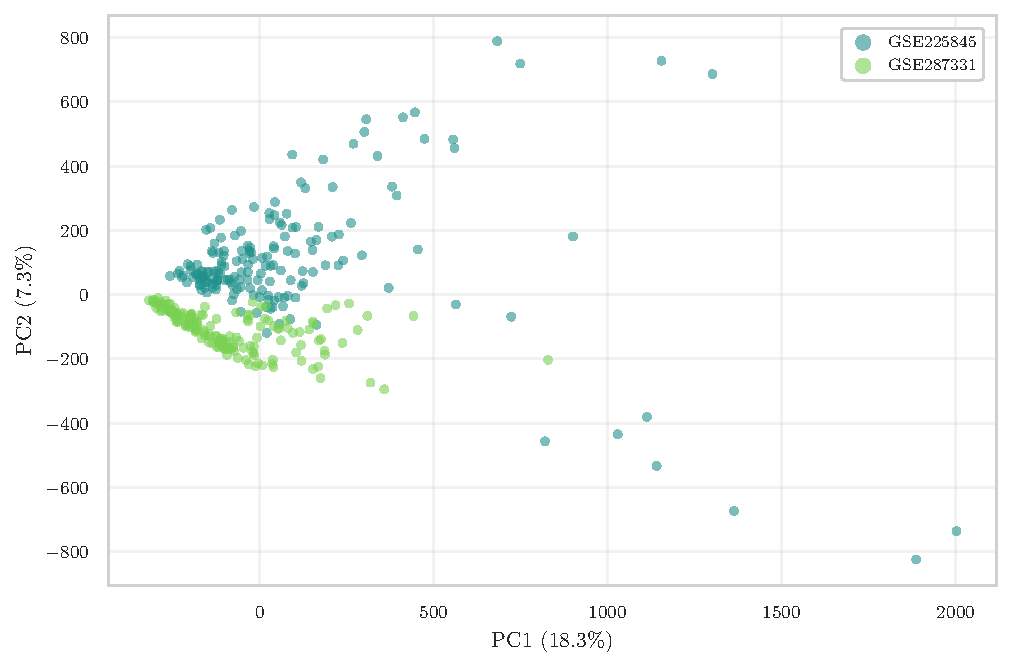
\includegraphics[width=\linewidth, height=2.9cm, keepaspectratio]{images/plot_pca_precombat_by_dataset.pdf}

\vspace{1pt}

{\scriptsize \textbf{Post-ComBat}}\\[2pt]
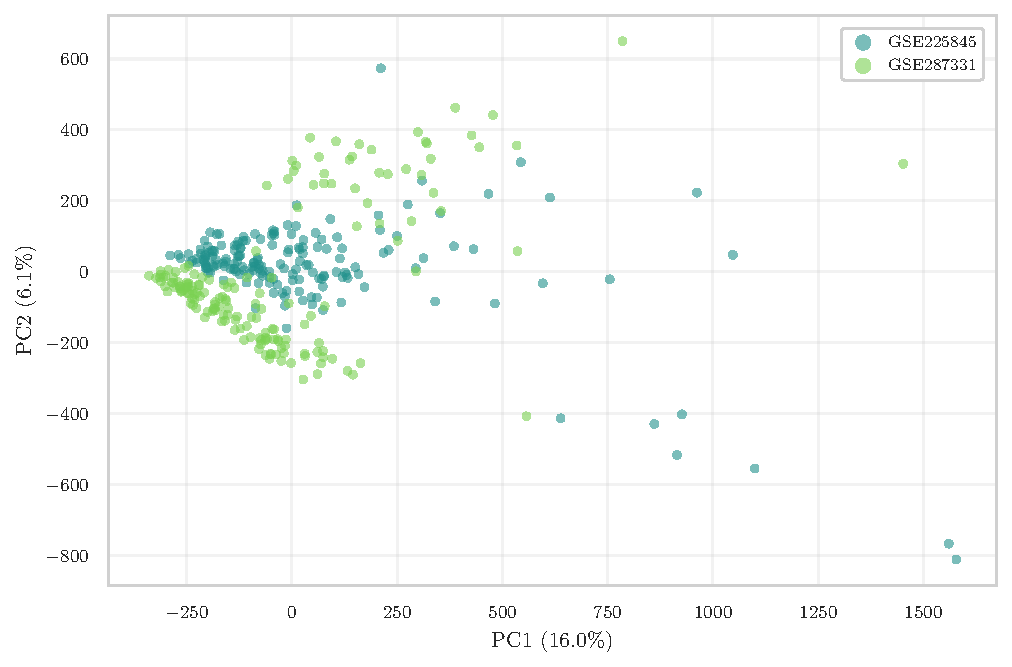
\includegraphics[width=\linewidth, height=2.9cm, keepaspectratio]{images/plot_pca_postcombat_by_dataset.pdf}

\end{columns}

\end{frame}

\begin{frame}{Appendice — Filtro di Variabilità (Edgar)}

\begin{columns}[c, onlytextwidth]

% ---- LEFT: formula ----
\column{0.42\textwidth}

{\footnotesize \textbf{Statistica di variabilità}}\\[0.6em]

{\small
\[
r_{\beta,j} = Q_{0.90}(\beta_j \mid \mathcal{D}_{\text{train}}) - Q_{0.10}(\beta_j \mid \mathcal{D}_{\text{train}})
\]
}

\vspace{0.6em}
{\scriptsize
Un CpG è ritenuto se e solo se:
\[
r_{\beta,j} \geq \tau, \quad \tau = 0.05
\]

\vspace{0.4em}
\begin{itemize}\setlength\itemsep{0.3em}
  \item \textbf{Filtro non supervisionato} — calcolato senza etichette di classe
  \item \textbf{Stimato solo su train} — applicato identicamente al test
  \item \textbf{Risultato:} 866k $\rightarrow$ $\sim$285k--485k CpG a seconda della coorte
\end{itemize}
}

% ---- RIGHT: immagine ----
\column{0.55\textwidth}
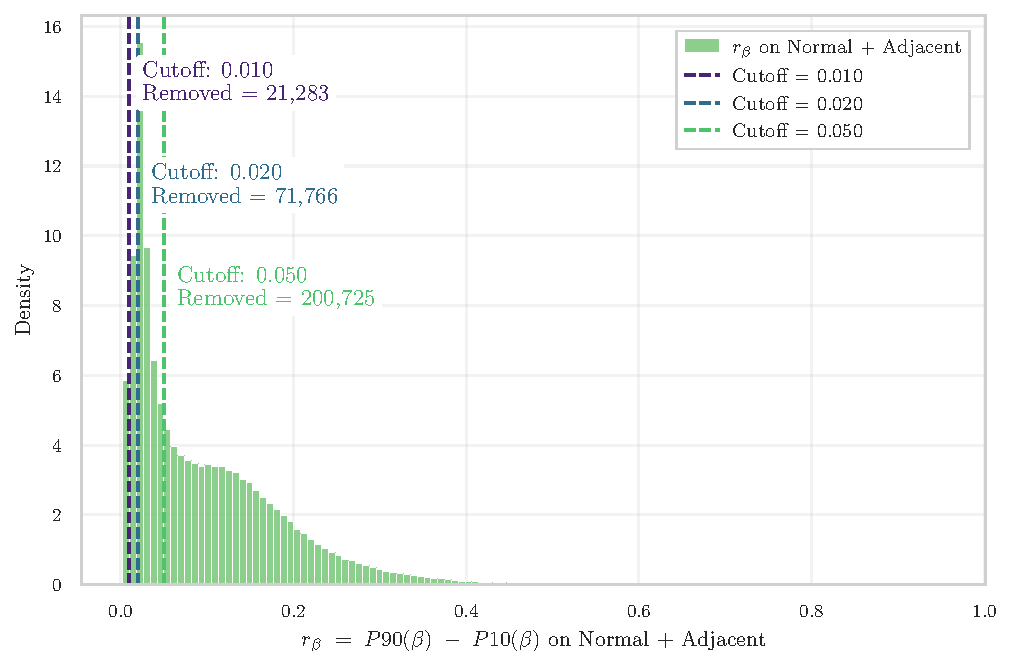
\includegraphics[width=\linewidth]{images/GSE287331_edgar_variability.pdf}

\end{columns}

\end{frame}
\begin{frame}{Appendice — Filtro Varianza in M-space}

\begin{columns}[c, onlytextwidth]

% ---- LEFT: formula ----
\column{0.42\textwidth}

{\footnotesize \textbf{Residual variance trimming}}\\[0.6em]

{\small
\[
\text{SD}_j = \sqrt{\frac{1}{n-1}\sum_{i=1}^{n}\bigl(M_{ij} - \bar{M}_j\bigr)^2}
\]
}

\vspace{0.6em}
{\scriptsize
Un CpG è rimosso se:
\(
\text{SD}_j < \text{SD}^*
\)

\vspace{0.4em}
\begin{itemize}\setlength\itemsep{0.3em}
  \item \textbf{Motivazione} — la mappa logit è non lineare: loci con $r_{\beta,j}$ basso ma concentrati ai bordi di $[0,1]$ producono M-value quasi costanti
  \item \textbf{Soglia data-driven} — primo minimo locale della distribuzione SD(M) sul train, che separa i loci quasi-costanti dallo spazio discriminativo principale
  \item \textbf{Risultato:} rimozione di $\sim$3k--8k CpG residui a seconda della coorte
\end{itemize}
}

% ---- RIGHT: immagine ----
\column{0.55\textwidth}
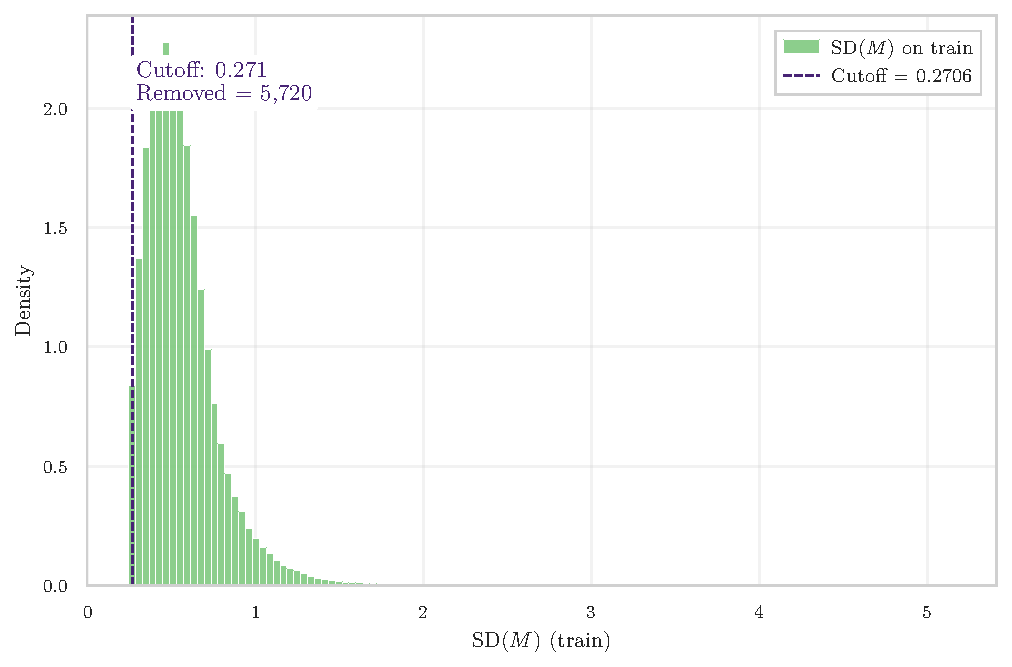
\includegraphics[width=\linewidth]{images/GSE287331_sdM_variance_filter.pdf}

\end{columns}

\end{frame}

\begin{frame}{Appendice — Diversificazione Genomica Vincolata}

\begin{columns}[c, onlytextwidth]

% ---- LEFT: formula ----
\column{0.42\textwidth}

{\footnotesize \textbf{Selezione greedy vincolata}}

{\scriptsize
\begin{alignat*}{2}
\min_{\mathcal{S} \subseteq \mathcal{R}} \quad
& \sum_{j \in \mathcal{S}} \text{score}_j \\
\text{s.t.} \quad
& |\mathcal{S}| = K_{\text{eff}} \\
& |\{j \in \mathcal{S} : c(j) = \chi\}| \leq \lfloor \alpha_{\text{chr}} K_{\text{eff}} \rfloor \quad \forall\,\chi \\
& |\{j \in \mathcal{S} : \gamma(j) = g\}| \leq \lfloor \alpha_{\text{ctx}} K_{\text{eff}} \rfloor \quad \forall\,g \\
& |\{j \in \mathcal{S} : w(j) = \omega\}| \leq B_\omega \quad \forall\,\omega
\end{alignat*}

con $\alpha_{\text{chr}} = 0.08$,\; $\alpha_{\text{ctx}} = 0.65$,\; $B_\omega = 15$.

\begin{itemize}\setlength\itemsep{0.3em}
  \item \textbf{Cardinalità} — esattamente $K = 5.000$ CpG
  \item \textbf{Cromosomica} — max 8\% per cromosoma
  \item \textbf{Contesto genomico} — max 65\% per classe (Island, Shore, OpenSea\ldots)
  \item \textbf{Finestra spaziale} — max 15 CpG per finestra da 500kb
\end{itemize}
}

% ---- RIGHT: immagine ----
\column{0.55\textwidth}
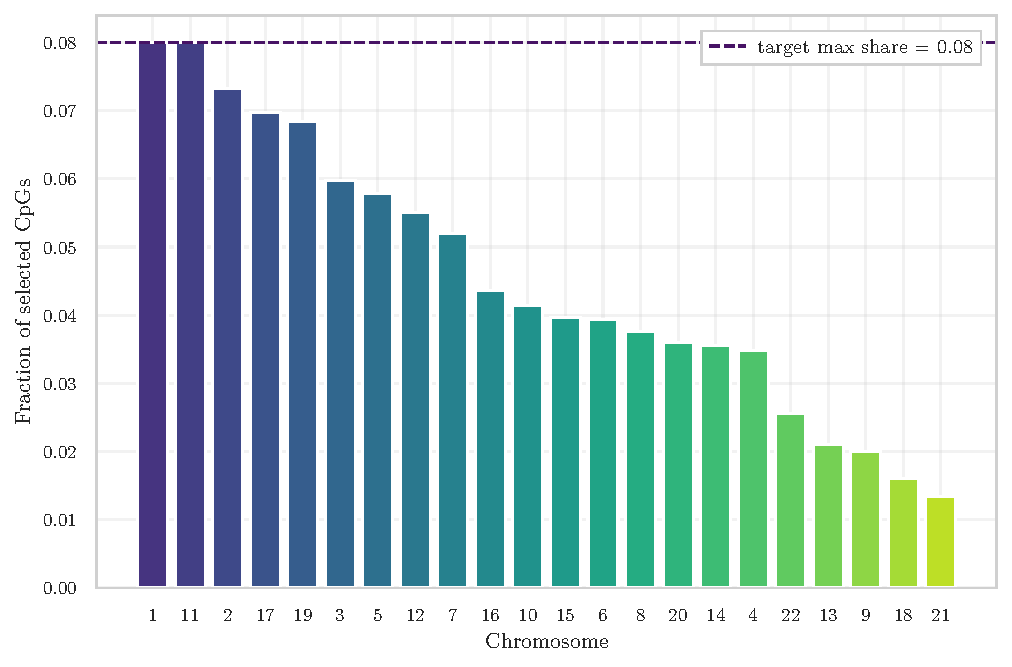
\includegraphics[width=\linewidth]{images/dataset_chromosome_share_diversified_K5000_maxfrac0.08.pdf}

\end{columns}

\end{frame}

\begin{frame}{Appendice — Formulazione completa MILP}
{\scriptsize
\begin{alignat*}{3}
\max_{x} \quad
& \underbrace{
    \sum_{j \in \mathcal{J}}
    \left(
      \underbrace{w_{\text{coef}}\,\tilde{c}_j}_{\text{coeff. SVM}}
      + \underbrace{w_{\Delta M}\,\tilde{d}_j}_{|\Delta M|}
      + \underbrace{w_{\sigma}\,\tilde{s}_j}_{\text{stabilità}}
      + \underbrace{w_{\text{COSMIC}}\,\mathbf{1}_{j \in \text{CGC}}}_{\text{gene noto}}
    \right) x_j
  }_{\text{score composito}}
  \;+\;
  \mu \cdot \underbrace{\frac{1}{K(2+\eta)}\!\left(
    \sum_{j:\,\text{prom}(j)} x_j
    + \sum_{j:\,\text{isl}(j)} x_j
    + \eta\sum_g y_g
  \right)}_{\hat{\Phi}(x,y)} & & \\[8pt]
\text{s.t.} \quad
& \sum_{j \in \mathcal{J}} x_j = 50
  \\[4pt]
& \sum_{j \in \mathcal{J}_c} x_j \leq 10 \quad \forall\, c
  \\[4pt]
& \sum_{j:\,g(j)=g} x_j \leq 2 \quad \forall\, g
  \\[4pt]
& x_j \leq y_{g(j)} \leq \textstyle\sum_{j':\,g(j')=g} x_{j'} \quad \forall\, j : g(j) \neq \emptyset
  \\[4pt]
& x_i + x_j \leq 1 \quad \forall\,(i,j):|r_{ij}|\geq 0.85
  \\[4pt]
& x_j,\, y_g \in \{0,1\}
\end{alignat*}
}
\end{frame}

\begin{frame}{Appendice — Estensione a una Diversa Piattaforma}

\begin{columns}[c, onlytextwidth]

% ---- LEFT: testo ----
\column{0.42\textwidth}

{\footnotesize \textbf{GSE69914 e GSE67919 — HM450K}}\\[0.3em]

{\scriptsize
Il pannello da 50 CpG è stato derivato su array \textbf{EPIC}.
L'estensione a HM450K introduce due limitazioni strutturali:

\vspace{0.3em}
\begin{itemize}\setlength\itemsep{0.2em}
  \item \textbf{Copertura ridotta} — HM450K interroga $\sim$450k sonde vs $\sim$866k di EPIC: non tutte le 50 CpG sono presenti su entrambi i dataset
  \item \textbf{Sonde non equivalenti} — le sonde condivise non sono garantite avere lo stesso comportamento chimico
  \item \textbf{Risultato} — le distribuzioni di $|\beta - \mu_{\text{Normal}}|$ su HM450K sono più larghe e meno separate rispetto alle coorti EPIC
\end{itemize}

\vspace{0.3em}
La validazione cross-piattaforma richiede una pipeline dedicata — identificata come sviluppo futuro.
}

% ---- RIGHT: immagine ----
\column{0.55\textwidth}
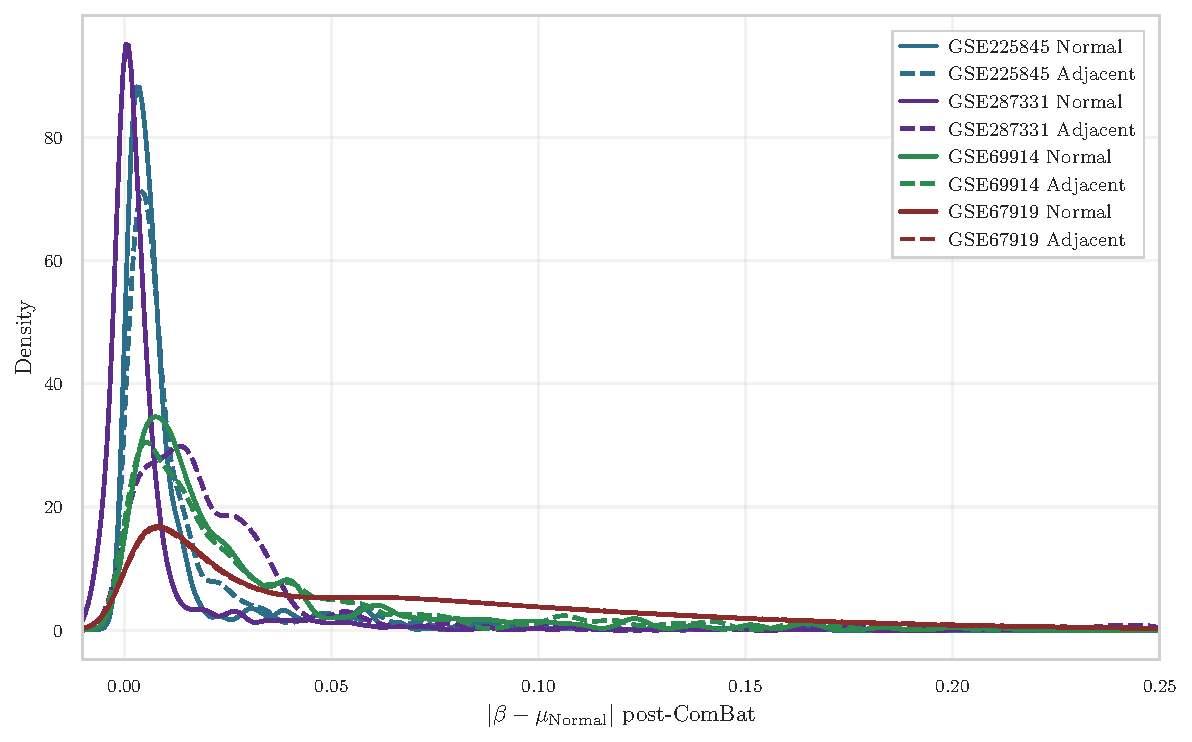
\includegraphics[width=\linewidth]{images/plot_abs_deviation_postcombat_4datasets (1).pdf}

\end{columns}

\end{frame}

\begin{frame}{Appendice — Tutti i Geni COSMIC nel Pannello}

\vspace{0.5em}
\centering
{\footnotesize
\renewcommand{\arraystretch}{1.2}
\begin{tabular}{llll}
\toprule
\textbf{Gene} & \textbf{Categoria} & \textbf{Gene} & \textbf{Categoria} \\
\midrule
RB1     & Tumor suppressor        & AKT1   & Segnalazione \\
TBX3    & Fattore di trascrizione & NOTCH1 & Segnalazione \\
NCOR1   & Regolatore cromatina    & MAP2K4 & Segnalazione \\
SMARCD1 & Regolatore cromatina    & FGF8   & Fattore di crescita \\
SALL4   & Fattore di trascrizione & WNT5A  & Segnalazione \\
PLEC    & Strutturale             & TYRO3  & Recettore tirosina kinasi \\
FBLN2   & Matrice extracellulare  &        & \\
\bottomrule
\end{tabular}
}

\vspace{0.5em}
{\scriptsize Fisher exact test (one-sided): arricchimento significativo
rispetto al background EPIC ($p < 0.001$).}

\end{frame}

\end{document}
